%%%%%%%%%%%%%%%%%%%%%%%%%%%%%%%%%%%%%%%%%
% Beamer Presentation
% LaTeX Template

\documentclass{beamer}
\mode<presentation> {
\usetheme{Warsaw}
}

\usepackage{multicol}
\usepackage[russian]{babel}
\usepackage{graphicx} 
\usepackage{hyperref}

\title[Introduction to Python]{Function, Class, Regular expressions \& other tools} 
\author{Sugarkhuu Radnaa} 
\institute[]
{
Py4Econ in Ulaanbaatar \\ 
\medskip
\textit{py4econ@gmail.com} 
}
\date{\today}  % 

\begin{document}

\begin{frame}
\titlepage % Print the title page as the first slide
\end{frame}

\begin{frame}
    \frametitle{Week 3: Learning objectives}
    Get to know: 
    \begin{enumerate}
        \item Functions and Modules
        \item Class (OOP basics)
        \item Regex 
        \item Additional
        \begin{itemize}
            \item One-liner & lambda
            \item Exception handling
            \item Debugging
        \end{itemize}         
    \end{enumerate}
\end{frame}

%------------------------------------------------
\section{Data types and structures} 
%------------------------------------------------

\begin{frame}
\frametitle{Function}
Function - not to repeat one action again and again
    \begin{center}
        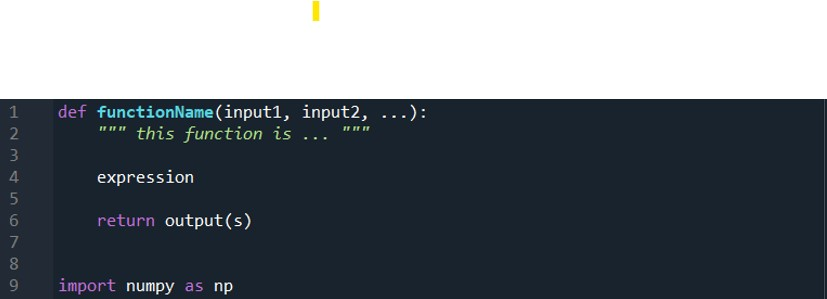
\includegraphics[scale=0.5]{figures/function.jpg}
    \end{center}        
\end{frame}

\begin{frame}
\frametitle{Documenting a function is crucial!}
Docstring prototype
        \begin{center}
            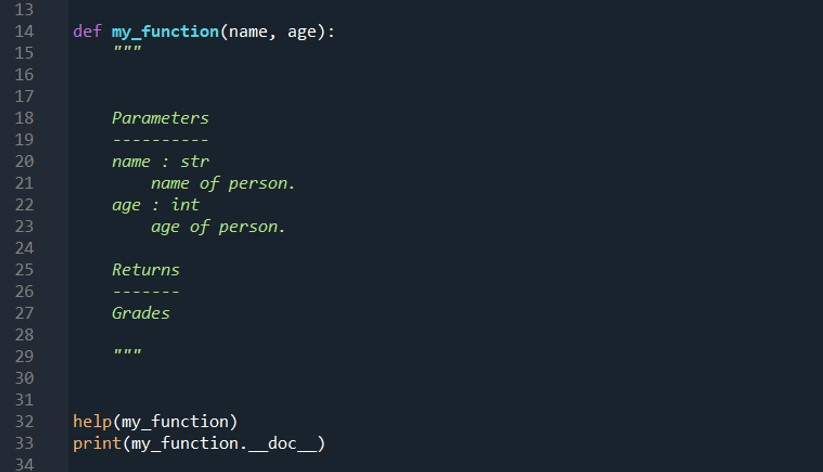
\includegraphics[scale=0.5]{figures/documentation.jpg}
        \end{center}
\end{frame}

\begin{frame}
\frametitle{Function arguments}
    \begin{itemize}
        \item Positional (“input”) 
        \item Keyword (“input=value”) - with a default value
        \item Optional positional (*args)
        \item Optional keyword (**kwargs)        
    \end{itemize}
\end{frame}


\begin{frame}
\frametitle{Scope of variable}
    \centering
    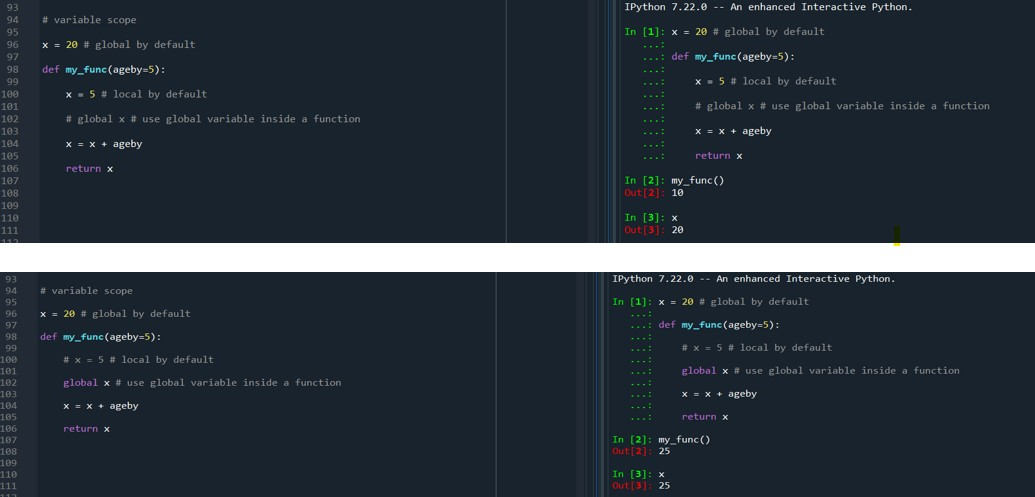
\includegraphics[scale=0.5]{figures/variable_scope.jpg}
\end{frame}

\begin{frame}
\frametitle{Module}

As your program gets longer, you may want
\begin{itemize}
    \item to split it into several files 
    for easier maintenance
    \item to use also a handy function that
    you have written in several programs without copying its definition into each 
    program.
\end{itemize}

\vskip 2mm 

To support this, Python has a way to put definitions in a file
and use them. Such a file is called a \textit{module}; definitions from 
a module can be imported into other modules or script. 

\end{frame}


\begin{frame}
\frametitle{Class – OOP philosophy}

\textbf{Def:} Object-oriented programming (OOP) is a computer programming 
model that organizes software design around data, or objects, 
rather than functions and logic. An object can be defined as a 
data field that has unique attributes and behavior.
\vskip 2mm 
Important concepts:
    \begin{itemize}
        \item Object (instance)
        \item Method
        \item Inheritance (super, child classes)
        \item Setters and getters
        \item Variable accessibility – Public/Private/Protected
    \end{itemize}
\end{frame}

\begin{frame}
\frametitle{One liner and Lambda}
    Helpful for writing concise codes
        \begin{center}
            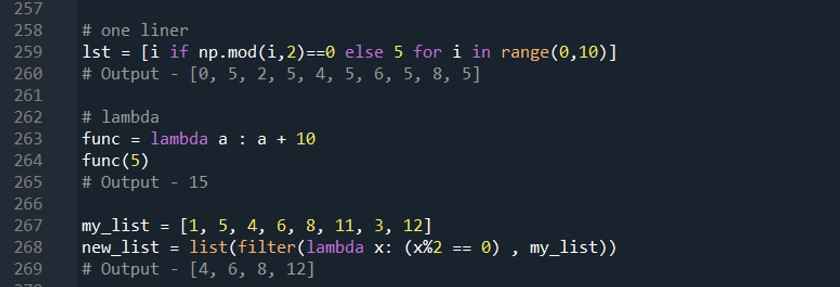
\includegraphics[scale=0.5]{figures/one_liner.jpg}
        \end{center}
\end{frame}

\begin{frame}
    \frametitle{Exception handling}
    Exceptions occur from time to time in any sort of job. 
    If you know what kind of errors potentially could occur
    and implement “remedy(ies)” on it beforehand
        \begin{center}
            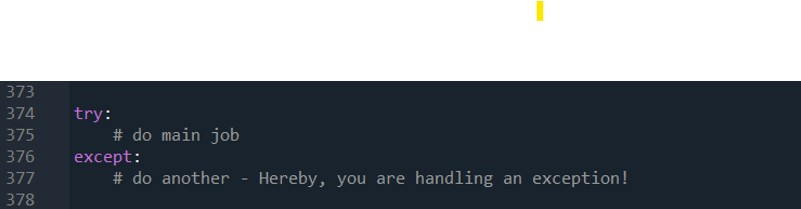
\includegraphics[scale=0.5]{figures/exception.jpg}
        \end{center}
\end{frame}

\begin{frame}
    \frametitle{Debugging}

In IDEs (VSCode):

    \begin{itemize}
        \item Actions at breakpoints: continue, step over, step into, step out
        \item Additional actions at breakpoints - expression, hit count, log message
        \item Watch
        \item Exceptions
    \end{itemize}

\vskip 2mm

Hand inputted breakpoint:

    \begin{itemize}
        \item import pdb, pdb.set\_trace()
    \end{itemize}
\end{frame}

\begin{frame}
    \frametitle{Regular expressions}
Search "pattern"  from text and do an action
Package “re”:
    \begin{itemize}
        \item compile
        \item findall – find all matches
        \item match – match at the beginning of string
        \item search – first match anywhere in string
        \item split – split string into pieces at pattern points
        \item sub – replace match by user input
        \item group 
        \item special characters
    \end{itemize}
\end{frame}

\begin{frame}
    \frametitle{Regular expressions special characters}
            \centering
            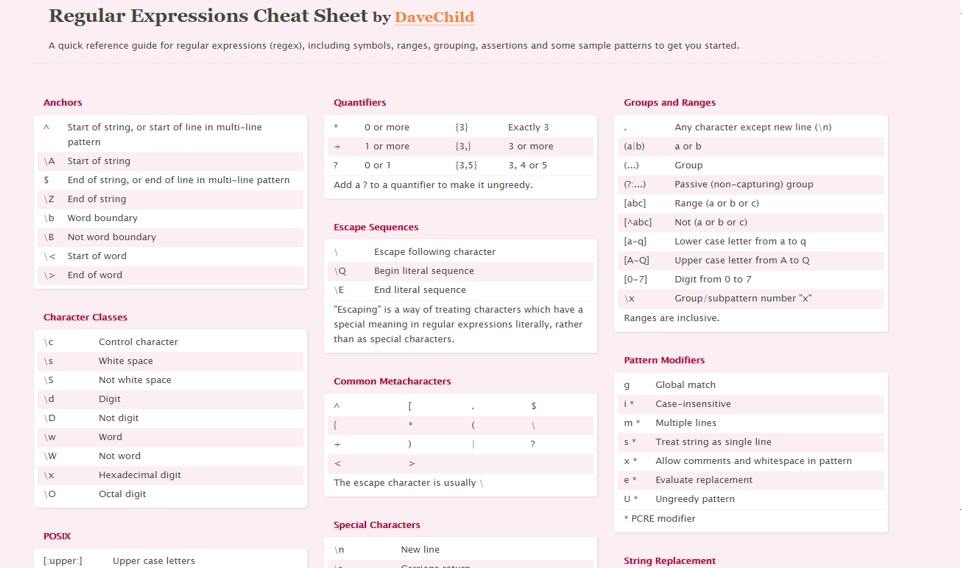
\includegraphics[scale=0.5]{figures/regex.jpg}
\end{frame}

\begin{frame}
    \frametitle{Additional reading: Why is “class” useful?}
    Please read most upvoted answer by "dantiston":
     \url{https://stackoverflow.com/questions/33072570/when-should-i-be-using-classes-in-python} 
\end{frame}

%------------------------------------------------
\section{Homework} 
%------------------------------------------------

\begin{frame}
    \frametitle{Homework}
    \begin{enumerate}
        \item Task 1
        \item Task 2
        \item Task 3
        \item Task 4
        \item Task 5
        \item Task 6
    \end{enumerate}

\vskip 2mm
Deadline: 31 December, 2021 \\

\vfill
\textbf{Note:} Create a github repo from the start and populate it with your results
\end{frame}

\begin{frame}
    \frametitle{Task 1: Function arguments}
    Jupyter notebook дээр зөвхөн args, зөвхөн args=value, зөвхөн *args, 
    зөвхөн **kwargs аргументуудтай (4 тусдаа функц) болон эдгээрийн холимог 
    (2 функц) байгуулж, ажиллуулж үзүүл. Нийт 6 функц.
\end{frame}

\begin{frame}
    \frametitle{Task 2: Class}
    Create a bank deposit class which you can 
    \begin{itemize}
        \item withdraw money
        \item deposit 
        \item check the balance
    \end{itemize}
    Show on Jupyter notebook how it works
\vskip 2mm
Examples: 
\tiny
    \begin{itemize}
        \item \url{https://www.engineeringbigdata.com/python-atm-code-for-account-balance-withdraw-and-deposit-functions/}
        \item \url{https://www.geeksforgeeks.org/python-program-to-create-bankaccount-class-with-deposit-withdraw-function/}
        \item \url{https://www.vtupulse.com/python-programs/python-program-using-classes-and-objects-to-deposit-and-withdraw-money-in-a-bank-account/}
        \item Tkinter GUI - \url{https://www.youtube.com/watch?v=SF-enJWjekY&list=PLtMugc7g4GapTtbhzODIjw7FJK-xJEBEE&index=16}
    \end{itemize}
\end{frame}

\begin{frame}
    \frametitle{Task 3: Exception}
    \begin{enumerate}
        \item Generate array of 1000 random integers in numpy and create an array with only the negative even numbers.
        \item Loop one by one through this array …
        \item \ldots when negative & odd, then raise “odd error” and continue to next loop, 
        \item \ldots when even but positive, raise “sign error” and continue to next loop \ldots
        \item \ldots when “negative even”, then append your list. 
    \end{enumerate}
\end{frame}

\begin{frame}
    \frametitle{Task 4: Debugging}
    \begin{itemize}
        \item Debugging гэж юу вэ?
        \item Breakpoint – ийн ямар 3 төрөл (log message г.м) Vscode дээр байдаг вэ?
        \item Debug-ийн step into, step over, stop out – ийн ялгааг тайлбарла 
    \end{itemize}
\end{frame}

\begin{frame}
    \frametitle{Task 5: Regex}
    Өөрөө зохиох эсвэл бэлэн текст интернетээс олж regex-ийн 
    дараах үйлдлүүдийг ашиглан текстүүд гаргаж авах жишээнүүд үзүүл 
    (нэг бүр дээр нь бус хамтад нь ашиглаж болно. Гэхдээ доорх бүх тэмдгээс ядаж 1 удаа ашиглаарай)

    \begin{itemize}
        \item {[a-zA-Z0-9], [a-z],[A-Z],[0-9]}
        \item \textbackslash d, \textbackslash D, \textbackslash w, \textbackslash W, \textbackslash s
        \item \^{}, \$, ?, *, +, .
        \item \{m,n\}, \{,n\}, \{m,\}, \{n\}
        \item Look behind, Look ahead, Negative look behind, Negative look ahead
    \end{itemize}
\end{frame}

\begin{frame}
    \frametitle{Task 6: Module}   
\tiny
    \begin{itemize}
        \item Өгсөн тоон list-ний нийлбэр, ялгавар, үржвэрийг олдог 3 тусдаа функц бүхий модуль файл үүсгэ. 
        \item Дээрх модульд “main” гэдэг функц нэм. Уг функц нь “жишээ” list-ний хувьд дээрх 3 функцийг ажиллуулан үр дүн гарч буйг хэвлэн гаргаж харуулдаг байна.
        \item if {\_\_name\_\_ == '\_\_main\_\_'}: дотор main() функцийг ажиллуулна (do something-ийн оронд байршин)
        \item python  “yourModuleName”.py гэж terminal дээр уншуулахад гарах үр дүн юу вэ? (screenshot байхад болно)
        \item Өөр файл дотроос “import yourModuleName” гэж импортлоход өмнөх хэсгийн үр дүнгүүд хэвлэгдэж гарахгүй байгаа. Яагаад?        
    \end{itemize}

\vskip 5 mm
    Check out on (answer of Fooz) "if \_\_name\_\_ == '\_\_main\_\_'": \\
    \url{https://stackoverflow.com/questions/419163/what-does-if-name-main-do}

\end{frame}

\begin{frame}
\Huge{\centerline{Thank you!}}
\end{frame}

%----------------------------------------------------------------------------------------

\end{document} 